
\subparagraph{Calcolo della capacità di un condensatore con MATLAB}
Si ricorda il modello dell'elettrostatica
$$
\begin{cases}
\nabla \times \vec{E} = 0 &\text{in } \Omega \Rightarrow \vec{E} = -\nabla u\\
\nabla\cdot\vec{D} = 0 &\text{in }\Omega\text{ non ci sono cariche libere}\\
\vec{D} = \varepsilon\vec{E} &\text{in } \Omega\text{ materiale omogeneo ed isotropo}
\end{cases}
$$
Il modello si trasforma in questo caso nel problema dei valori al contorno
per l'equazione di Laplace con condizioni di Dirichlet sugli elettrodi
e condizione alla Neumann su una frontiera abbastanza lontana da approssimare
l'infinito.
$$
\begin{cases}
\nabla^2 u = 0 & \text{in } \Omega\\
\left.u\right|_{l_1} = V_1\\
\left.u\right|_{l_2} = 0\\
\left.\frac{\partial u}{\partial n}\right|_{\partial\Omega e} = 0
\end{cases}
$$
Le funzioni ``tenda'' solitamente utilizzate nei metodi agli elementi finiti
sono lineari a tratti, ad esempio la funzione $w_i$ vale $1$ nel nodo
in cui è valutata e decresce linearmente a $0$ nei nodi adiacenti.
Il grado del polinomio della funzione test può essere incrementato ma
si incrementano anche i problemi analitici dovuti al rispetto
delle condizioni al contorno e di raccordo, per questo motivo sono solitamente
utilizzati polinomi di grado 1.
\begin{figure}[H]
\centering
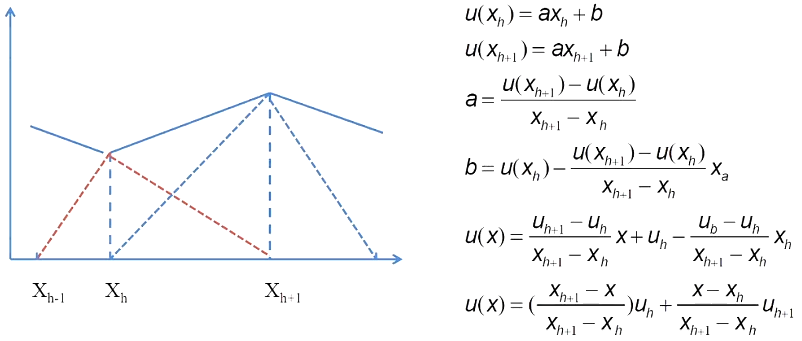
\includegraphics[width=0.7\linewidth]{funzione_tenda}
\caption{Espressione analitica funzione tenda di grado 1}
\end{figure}
Per ricostruire la funzione si esegue una combinazione lineare delle
funzioni tenda nei vari punti.

Per domini bidimensionali è ancora possibile eseguire una discretizzazione
in elementi triangolari, con funzioni lineari in due variabili,
la matrice dei coefficienti risultante è simmetrica e semidefinita
positiva, inoltre è una matrice sparsa, ossia i coefficienti pari a zero sono 
molto maggiori rispetto a quelli diversi da zero, ciò è vantaggioso
durante il calcolo del prodotto matriciale, necessario alla risoluzione
del problema.
\begin{figure}[H]
\centering
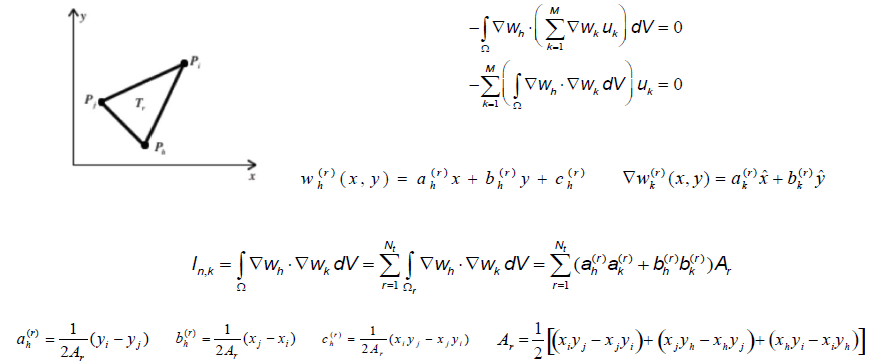
\includegraphics[width=0.7\linewidth]{tenda_bidimensionale}
\caption{Espressione funzione tenda bidimensionale}
\end{figure}

Per impostare un problema con il \textit{pdetool} è necessario
seguire i seguenti passaggi:
\begin{enumerate}
\item Definizione del problema fisico e del suo modello matematico
\item Definizione della geometria con ausilio di CAD
\item Imposizione delle condizioni al contorno
\item Discretizzazione del dominio (\textit{meshing}), l'errore aumenta
all'aumentare dell'irregolarità dei triangoli
\item Si assegnano le matrici dei termini noti e si risolve il sistema lineare
\end{enumerate}

\subparagraph{Dominio bucato con pdetool}
Si riassumono brevemente gli step da eseguire per studiare un dominio quadrato
al quale vengono sottratte due circonferenze ad esso interne.

Si piazzano e si disegnano il rettangolo e le circonferenze, è poi
fondamentale impostare la ``formula'' del dominio, ossia la pseudo-equazione
che descrive logicamente il dominio da analizzare; in questo caso si sta
trattando un quadrato bucato, chiamato $R1$ il rettangolo e $E1$ ed $E2$ 
le due circonferenze, la ``formula'' sarà quindi $R1-E1-E2$.

Definita la geometria vanno assegnate le condizioni al contorno mediante il menù ``Boundary'' e impostare le condizioni di Dirichlet per specificare
ad esempio il potenziale di quel lato a 0 oppure 1 e -1 sugli elettrodi
sferici.

In ``PDE'' è possibile specificare la costante dielettrica relativa del
dominio e la densità di carica libera al suo interno, questi due valori
nell'esempio sono stati posti rispettivamente a 1 e 0.

Si può ora procedere al meshing del dominio eseguendo successivamente
un numero appropriato di ``raffinamenti'' ossia di riduzioni delle
dimensioni degli elementi.

Premendo sul pulsante '$=$' è possibile risolvere il problema, il risolutore
mostrerà di default il potenziale con una scala di colori. Cambiando le 
impostazioni è possibile rappresentare diverse grandezze, aggiungere 
isolinee del potenziale o linee di forza del campo.
\newpage
Si ottiene un risultato simile:
\begin{figure}[H]
\centering
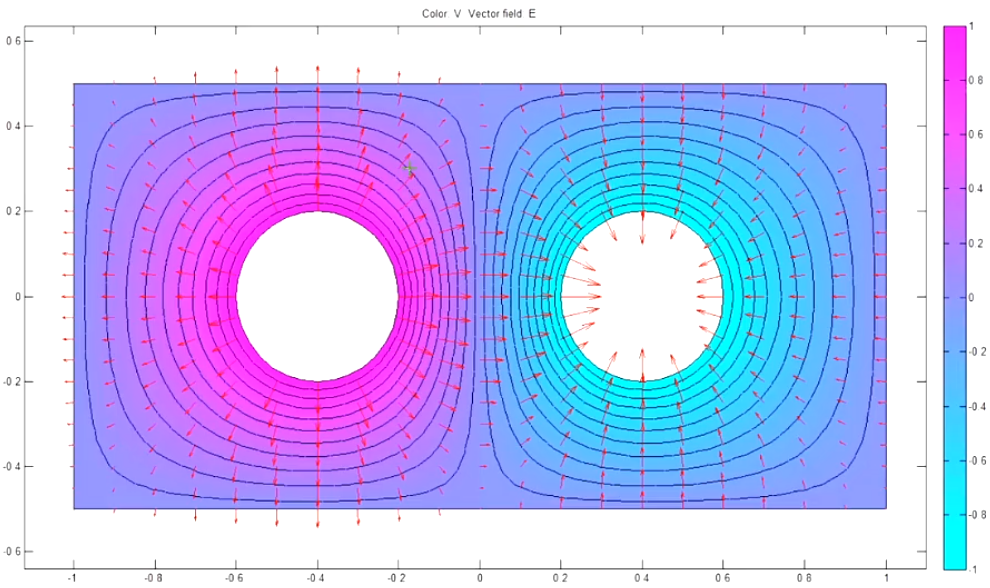
\includegraphics[width=0.8\linewidth]{potenziale_due_conduttori_FEM}
\caption{Potenziale e vettori forza prodotti da due conduttori carichi}
\end{figure}

È possibile utilizzare il \textit{pdetool} mediante la riga di comando
o uno script MATLAB
\begin{lstlisting}[style=Matlab-editor,language = Matlab]
%Definizione del rettangolo
pderect([xmin xmax ymin ymax],'R1');
%Definizione della circonferenza
pdecirc(xc,yc,r,'E1');
%Impostazione della set formula
set(findobj(get(pde_fig,'Children'),'Tag','PDEEval'),'String','R1-E1');
%Esportazione della geometria
bl=get(findobj(get(pde_fig,'Children'),'flat','Tag','PDEBoundMenu'),'UserData');
%Impostazioned elle boundary
%Neumann
pdesetbd(5,'neu',1,'0','0');
%Dirichlet, V e' la variabile stringa del potenziale num2str(10)
pdesetbd(4,'dir',1,'1',V);
%Generazione della MESH
[p1,e1,t1]=initmesh(dl,'Hmax',0.01,'init','off');
%rifinitura
[p,e,t]=refinemesh(dl,p1,e1,t1,'regular');
%Plot della MESH
pdeplot(p,e,t);
\end{lstlisting}
I numeri indicati nel comando ``pdesetbd'' si possono ricavare dal menù
Boundary $>$ Show Edge Labels, corrispondono all'identificativo del lato
del dominio.

La matrice $p$ contiene le coordinate dei nodi della mesh.

La matrice $e$
contiene i nodi del contorno, le prime due righe contengono gli indici
dei nodi iniziali e finali dei segmenti del contorno, la terza e la quarta
contengono i valori iniziali e finali del parametro, la quinta contiene
il numero identificativo del segmento di frontiera, la sesta e la settima
contengono i numeri dei sottodomini a destra e sinistra del segmento.

La matrice $t$ o matrice dei triangoli fornisce la relazione di appartenenza tra 
nodi e triangoli, la n-esima colonna coincide con l'n-esimo triangolo e contiene
la terna antioraria degli indici dei nodi dei suoi vertici.

Verificata la coerenza della mesh è possibile assemblare il problema e risolverlo
\begin{lstlisting}[style=Matlab-editor,language = Matlab]
u=assempde(bl,p,e,t,c,a,f);
\end{lstlisting}

\subsection{Capacità di un condensatore con FEM}
Si definiscono le equazioni del problema
$$
\begin{cases}
\nabla^2u = 0\\
\left. u\right|_{l_1} = 10\\
\left. u\right|_{l_2} = 0\\
\left.\frac{\partial u}{\partial n}\right|_{\text{inf}} = 0
\end{cases}
\Rightarrow
\begin{cases}
\frac{1}{\rho}\left(\frac{\partial}{\partial \rho}\left(\rho\frac{\partial}{\partial\rho}u\right)+
\frac{\partial}{\partial z}\left(\rho\frac{\partial}{\partial z}u\right)\right)=0\\
\left. u\right|_{l_1} = 10\\
\left. u\right|_{l_2} = 0 \\
\rho\left.\frac{\partial u}{\partial n}\right|_{\text{inf}} = 0
\end{cases}
$$
\begin{figure}[H]
\centering
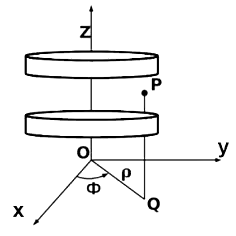
\includegraphics[width = 0.25\linewidth]{geom_condensatore_FEM}
\caption{Geometria condensatore con armature cilindriche}
\end{figure}
Il sistema è simmetrico rispetto all'asse $z$ e il problema
viene formulato mediante coordinate polari.
All'aumentare del raggio dei dischi, il condensatore si comporta come
un condensatore piano indefinito, trascurando gli effetti di bordo,
allontanandosi dal dispositivo invece si vede come il campo prodotto
all'esterno sia simile a quello di un dipolo.
\newpage
Sfruttando la simmetria della struttura è possibile analizzare il problema
studiandone metà, questo permette di ridurre i costi computazionali data la
dimensione ridotta della mesh.
\begin{lstlisting}[style=Matlab-editor,language = Matlab]
%definizione coordinate
xmin=0;
xmax=0.1;
ymin=-0.1;
ymax=0.1;
%Spessore dielettrico
dh=7.5e-4;
%Costante dielettrica relativa
epsr=2.9;
%Definizione rettangoli rappresentanti le armature
pderect([xmin xmax dh/2 ymax],'R1');
pderect([xmin xmax -dh/2 ymin],'R2');
%Dominio esterno
pderect([1.5*xmin 1.5*xmax 5*ymin 5*ymax],'R3');
%Impostazione regola dominio (set string)
set(findobj(get(pde_fig,'Children'),'Tag','PDEEval'),'String','R3-R2-R1');
%Esportazione dominio
dl=get(findobj(get(pde_fig,'Children'),'flat','Tag','PDEBoundMenu'),'UserData');
\end{lstlisting}
Si impongono le condizioni di Neumann sul dominio esterno, mentre quelle di 
Dirichlet sulle due armature, impostando due potenziali arbitrari.

Si esegue il meshing
\begin{lstlisting}[style=Matlab-editor,language = Matlab]
[p1,e1,t1]=initmesh(dl,'Hmax',0.1,'init','off');
[p,e,t]=refinemesh(dl,p1,e1,t1,'regular');
%Coordinata rho del baricentro dei triangoli
x=pdeinterp(p,t,p(1,:)');
%Calcolo soluzione
u=assempde(dl,p,e,t,x,'0','0');
\end{lstlisting}
Si vede che la mesh è molto disuniforme, molto fitta tra le armature e meno
all'esterno e verso i bordi. Per calcolare la capacità si valuta l'energia
immagazzinata, ricordando che in questo caso $v=Ed$
$$
w_e(t) = \frac{1}{2}Cv(t)^2 = \frac{1}{2}\varepsilon\frac{S}{d}v(t)^2 = 
\frac{1}{2}\varepsilon SdE^2
$$
Conoscendo il campo elettrico nel volume tra le due armature
$$
\frac{1}{2}Cv^2 = \iiint_{\mathbb{R}^3}\varepsilon \frac{E^2}{2}dV
$$
Conoscendo il secondo termine dalle simulazioni e la tensione imposta, si ricava
facilmente la capacità.
$$
\text{Energia } = \frac{1}{2}\varepsilon\cdot\int_0^{2\pi} d\theta 
\int_{zmin}^{zmax}\int_0^{\rho max} \left|E(r,z)\right|^2\cdot \rho\ d\rho\ dz =
\frac{1}{2}C\Delta V^2
$$
$$
C = \frac{\varepsilon\cdot \int_0^{2\pi} d\theta 
\int_{zmin}^{zmax}\int_0^{\rho max} \left|E(r,z)\right|^2\cdot \rho\ d\rho\ dz}{\Delta V^2}
$$
Risolvendo il calcolo su MATLAB
\begin{lstlisting}[style=Matlab-editor,language = Matlab]
[UX,UY] = pdegrad(p,t,u);
%Numero dei triangoli
Nt = size(t,2);
%area di ogni triangolo
area = abs(pdetrg(p,t));    

Energia = 0;
for n = 1:Nt     
    E2 = (UX(n)^2+UY(n)^2);  %norm(E)^2
    Energia = Energia+0.5*eps0*E2*area(n)*1;
end

%Capacita' teorica e numerica
Cteor = eps0*height*1/dist
Cnum = 2*Energia/(v1-v2)

%Errore relativo
e_rel = (Cnum-Cteor)/Cteor
\end{lstlisting}
È possibile visualizzare analoghe simulazioni negli appunti in pdf
su questa lezione.

\subparagraph{Risolutore circuiti simbolico}
Al seguente link \href{http://143.225.92.177:54323/}{tinyurl.com/ss2lcsmda}
è possibile vedere un solutore di circuiti simbolico che sfrutta la 
trasformata di Laplace e fornisce la soluzione nel dominio del tempo.
Il seguente circuito d'esempio deve essere trasformato in \textit{netlist} per 
essere risolto con il software.
\begin{figure}[H]
\centering
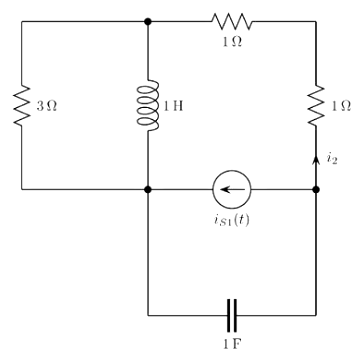
\includegraphics[width = 0.3\linewidth]{circuito_risolutore_simbolico}
\caption{Esempio circuito da risolvere con il risolutore}
\end{figure}
La netlist si può generare in questo modo:
\begin{lstlisting}
J 0 1 delta(t)
C 1 0 1
L 1 2 1
R1 1 2 3
R2 2 3 1
ZO 0 3 1
\end{lstlisting}
1:36:11

